\documentclass[12pt]{article}

\usepackage{sbc-template}
\usepackage{graphicx,url}
\usepackage[utf8]{inputenc}
\usepackage[brazil]{babel}
\usepackage{amsmath}
\usepackage{algorithm}    
\usepackage{algpseudocode}  
\usepackage{float}
\usepackage{booktabs}

\sloppy

\title{Trabalho Prático 2 \\ Algoritmos 2 2026/2}

    \author{Marney Santos de Melo - 2024106034 \\ Rafael Augusto Miranda 2024065990 \\ Victor Murilo Kaizer 2024096551}


\address{Instituto de Ciências Exatas \\ Departamento de Ciência da Computação \\ Universidade Federal de Minas Gerais
  (UFMG)\\
  \email{marneymelo@ufmg.br, rafaelrmiranda@ufmg.br,
  victor@ufmg.br}
}

\begin{document} 

\maketitle
     
\begin{abstract}
  This paper presents an empirical study of three algorithms for the
  Euclidean/metric Traveling Salesman Problem (TSP): an exact
  Branch-and-Bound, the Twice-around-the-tree approximation and
  Christofides' algorithm. Using 14 TSPLIB instances ($14 \le N \le 70$)
  and a 30-minute limit per run, we profile subroutines, fit asymptotic
  models, measure the effect of five warm-start strategies on the search
  tree, and relate instance features to solution quality. The root lower
  bound gap explains the exact algorithm's collapse better than $N$ alone,
  and warm-starts yield only modest pruning gains under a greedy DFS.
\end{abstract}

\begin{resumo}
  Este artigo apresenta um estudo empírico de três algoritmos para o
  Problema do Caixeiro Viajante (TSP) métrico: um Branch-and-Bound exato,
  o aproximativo Twice-around-the-tree e o algoritmo de Christofides.
  Com 14 instâncias da TSPLIB ($14 \le N \le 70$) e limite de 30 minutos
  por execução, realizamos profiling por subrotina, ajustamos modelos
  assintóticos, medimos o efeito de cinco estratégias de \textit{warm-start}
  na árvore de busca e relacionamos características das instâncias à
  qualidade das soluções. A folga do limite inferior na raiz explica o
  colapso do algoritmo exato melhor que $N$ isoladamente, e o
  \textit{warm-start} gera ganhos modestos de poda sob uma DFS gulosa.
\end{resumo}


\section{Introdução}

O Problema do Caixeiro Viajante (TSP) consiste em encontrar o ciclo hamiltoniano de menor custo em um grafo completo ponderado. Por ser NP-difícil, é um bom caso para comparar algoritmos exatos, que garantem o ótimo mas têm custo exponencial, com algoritmos aproximativos, que são rápidos e têm garantia de qualidade para custos métricos: fator 2 no \textit{Twice-around-the-tree} e fator $1{,}5$ no de Christofides.

Neste trabalho, auditamos e instrumentamos um \textit{Branch-and-Bound} exato (DFS com limite inferior via MST), o \textit{Twice-around-the-tree} e o algoritmo de Christofides, usando 14 instâncias da TSPLIB com $14 \le N \le 70$ e limite de 30 minutos por execução. Avaliamos o profiling por subrotina e o ajuste de modelos assintóticos, o impacto de cinco estratégias de \textit{warm-start} na árvore de busca e a influência de características geométricas das instâncias na qualidade das soluções. Parte do código foi gerada com auxílio de IA, e as refatorações aplicadas são descritas ao longo do texto.



\section{Algoritmo aproximativo: Twice-around-the-tree}
Um dos algoritmos aproximativos mais comuns para o problema do caixeiro viajante é o Twice-Around-The-Tree, com um fator de aproximação $\alpha = 2$. Note que, esse algoritmo exige que a instância do TSP seja Euclidiano, ou seja, que respeite a desigualdade triangular.

A ideia dele é basicamente encontrar uma Árvore Geradora Mínima (MST) e então duplicar as arestas, para que seja possível sair e voltar daquele vértice. No entanto, isso resultaria em visitar o mesmo vértice mais de uma vez, por isso, sempre que formos passar por um vértice repetido, nós atalhamos e optamos pelo caminho direto (desigualdade triangular).  O pseudo-código do algoritmo é basicamente:

% Preâmbulo
\floatname{algorithm}{Algoritmo}
\renewcommand{\algorithmicrequire}{\textbf{Entrada:}}
\renewcommand{\algorithmicensure}{\textbf{Saída:}}
\renewcommand{\algorithmicreturn}{\textbf{retorne}}

% Corpo
\begin{algorithm}[H]
\caption{Approx-TSP-Tour$(G, c)$}
\begin{algorithmic}
\Require grafo completo $G=(V,E)$ e função de custo $c$ (métrica)
\Ensure ciclo hamiltoniano $H$
\State selecione um vértice $r \in G.V$ para ser a raiz
\State calcule uma árvore geradora mínima $T$ de $G$ a partir da raiz $r$
\State seja $H$ a lista de vértices ordenados pela primeira visita
       em um percurso em pré-ordem de $T$
\State \Return o ciclo hamiltoniano $H$
\end{algorithmic}
\end{algorithm}

\subsection{Implementação e Auditoria do Código}
A implementação do algoritmo foi realizada com ajuda de IA, que montou um esqueleto a partir do pseudo-código fornecido a ela:
\begin{itemize}
    \item Para calcularmos a Árvore Geradora Mínima (MST), optamos por utilizar o algoritmo de Prim, que nos retorna uma árvore com as arestas de menor custo em tempo $O(N^2)$, com $N$ sendo o número de vértices. Note que como o gráfico do TSP é completo, é melhor usar o Prim do que o Kruskal, já que o Kruskal terá $|E| = \frac{N(N-1)}{2}$.
    \item Percorremos a árvore em pré-ordem, de forma iterativa. Isso porque, com grandes instâncias, o recursão do Python pode chegar a um limite e crashar.
    \item Temos também uma função para calcular o ciclo, com complexidade linear de $O(N)$.
\end{itemize}

Cada uma das subrotinas é chamada de forma que o seu tempo é marcado e salvo em uma planilha. Isolamos o coletor de lixo, pegamos o tempo no instante $t_0$, executamos a subrotina, e então subtraímos o tempo de término da subrotina para encontrar o tempo de execução: $t_f - t_i = t_{subrotina}$. Veremos a seguir os resultados dos testes empíricos.

\subsection{Resultados Experimentais e Modelagem Assintótica}
Podemos notar que ao executar o algoritmo, obtemos um gap de otimalidade dentro do esperado: todas as soluções são no máximo, duas vezes pior que o valor ótimo da instância TSP, para instâncias métricas. Ainda que o limiar não seja garantido nas outras instâncias, os valores de gap ainda são completamente aceitáveis É possível visualizar isso na coluna de Gap (\%).
% Requer no preambulo: \usepackage{booktabs}  (e \usepackage{float} se usar [H])
\begin{table}[H]
\centering
\label{tab:twice-qualidade}
\begin{tabular}{l|r|l|r|r|r}
\toprule
Instância & $n$ & Tipo & Custo & Ótimo & Gap (\%) \\
\hline

\midrule
burma14 & 14 & GEO & 3814 & 3323 & 14.78 \\
ulysses16 & 16 & GEO & 7903 & 6859 & 15.22 \\
gr17 & 17 & EXPLICIT & 2352 & 2085 & 12.81 \\
gr21 & 21 & EXPLICIT & 3728 & 2707 & 37.72 \\
ulysses22 & 22 & GEO & 8401 & 7013 & 19.79 \\
gr24 & 24 & EXPLICIT & 1607 & 1272 & 26.34 \\
fri26 & 26 & EXPLICIT & 1112 & 937 & 18.68 \\
bays29 & 29 & EXPLICIT & 2370 & 2020 & 17.33 \\
dantzig42 & 42 & EXPLICIT & 894 & 699 & 27.90 \\
swiss42 & 42 & EXPLICIT & 1641 & 1273 & 28.91 \\
att48 & 48 & ATT & 13925 & 10628 & 31.02 \\
eil51 & 51 & EUC\_2D & 581 & 426 & 36.38 \\
berlin52 & 52 & EUC\_2D & 10114 & 7542 & 34.10 \\
st70 & 70 & EUC\_2D & 888 & 675 & 31.56 \\
\bottomrule
\end{tabular}
\caption{Qualidade das soluções do \textit{Twice-Around-the-Tree}: custo obtido, ótimo conhecido e \textit{gap} percentual.}
\end{table}

Agora, analisando as subrotinas, é possível ver que o tempo de execução do algoritmo é quase que completamente dominado pela execução do Prim, para encontrar a árvore geradora mínima. A mesma coisa vale para a memória, em que ocupa mais espaço do que qualquer outra subrotina do Twice-Around-The-Tree.

\begin{table}[H]
\centering
\label{tab:twice-recursos}
\resizebox{\linewidth}{!}{%
\begin{tabular}{l|r|r|r|r|r|r|r|r}
\toprule
 & & \multicolumn{4}{c}{Tempo (ms)} & \multicolumn{3}{c}{Memória (KB)} \\
\hline
\cmidrule(lr){3-6}\cmidrule(lr){7-9}
Instância & $n$ & MST & Pré-ordem & Custo & Total & MST & Pré-ordem & Total \\
\hline
\midrule

burma14 & 14 & 0.156 & 0.012 & 0.014 & 0.182 & 5.86 & 0.38 & 6.07 \\
ulysses16 & 16 & 0.336 & 0.019 & 0.033 & 0.399 & 6.38 & 0.37 & 6.59 \\
gr17 & 17 & 0.339 & 0.022 & 0.031 & 0.404 & 6.69 & 0.41 & 6.89 \\
gr21 & 21 & 0.356 & 0.018 & 0.028 & 0.423 & 7.63 & 0.41 & 7.84 \\
ulysses22 & 22 & 0.280 & 0.015 & 0.021 & 0.324 & 7.85 & 0.43 & 8.05 \\
gr24 & 24 & 0.284 & 0.016 & 0.023 & 0.338 & 8.30 & 0.48 & 8.51 \\
fri26 & 26 & 0.331 & 0.021 & 0.024 & 0.367 & 8.86 & 0.48 & 9.06 \\
bays29 & 29 & 0.462 & 0.022 & 0.028 & 0.510 & 9.46 & 0.54 & 9.67 \\
dantzig42 & 42 & 0.509 & 0.027 & 0.030 & 0.575 & 12.73 & 0.66 & 12.93 \\
swiss42 & 42 & 0.519 & 0.024 & 0.029 & 0.581 & 12.79 & 0.65 & 13.00 \\
att48 & 48 & 0.614 & 0.025 & 0.034 & 0.667 & 14.07 & 0.70 & 14.27 \\
eil51 & 51 & 0.704 & 0.031 & 0.038 & 0.773 & 14.87 & 0.70 & 15.07 \\
berlin52 & 52 & 0.686 & 0.031 & 0.040 & 0.761 & 15.20 & 0.66 & 15.41 \\
st70 & 70 & 0.590 & 0.025 & 0.032 & 0.652 & 19.57 & 0.88 & 19.77 \\
\bottomrule
\end{tabular}}
\caption{Tempo (ms) e pico de memória (KB) do \textit{Twice-Around-the-Tree}, medidos com 20 repetições, por etapa (MST, pré-ordem e cálculo do custo).}

\end{table}

\subsection{Modelagem Assintótica e Discussão Crítica}
Para modelar a complexidade em função de $N$, ajustamos curvas teóricas aos dados da tabela por regressão não linear (\texttt{scipy.optimize.curve\_fit}), com $R^2$ e RMSE calculados pelo \texttt{scikit-learn}. Para cada subrotina comparamos o modelo teórico esperado com alternativas, usando também o AICc, que penaliza o número de parâmetros em amostras pequenas (aqui, 14 instâncias).

\begin{table}[H]
\centering
\label{tab:twice-regressao}
\begin{tabular}{l|l|r|r}
\toprule
Grandeza / Subrotina & Modelo & $R^2$ & RMSE \\
\midrule
Tempo, MST          & $aN^2 + c$ (teórico) & 0{,}648 & 0{,}096 ms \\
Tempo, MST          & $aN + c$             & 0{,}774 & 0{,}077 ms \\
Tempo, Pré-ordem    & $aN + c$             & 0{,}586 & 0{,}0035 ms \\
Tempo, Custo        & $aN + c$             & 0{,}396 & 0{,}0051 ms \\
Tempo, Total        & $aN + c$             & 0{,}755 & 0{,}084 ms \\
\midrule
Memória, MST        & $aN + c$             & 0{,}9998 & 0{,}053 KB \\
Memória, Pré-ordem  & $aN + c$             & 0{,}975  & 0{,}024 KB \\
Memória, Custo      & constante ($\approx 0{,}227$ KB) & -- & 0 KB \\
Memória, Total      & $aN + c$             & 0{,}9998 & 0{,}053 KB \\
\bottomrule
\end{tabular}
\caption{Ajustes de regressão por subrotina (instâncias TSPLIB, $14 \le N \le 70$).}
\end{table}

Uma das principais observações a se fazer é que a memória cresce de forma linear com o número de vértices e, assim como vimos na seção anterior, é completamente dominada pelo algoritmo responsável por encontrar a MST.

\begin{figure}[H]
    \centering
    \includegraphics[width=0.75\linewidth]{memória.png}
    \label{fig:placeholder}
\end{figure}

No entanto, durante a montagem do projeto, foi identificado que havia uma cópia desnecessária na matriz de pesos usada no algoritmo de Prim. Isso causou um grande gargalo: como copiávamos a matriz, nossa complexidade de espaço atingia $O(N^2)$ quando faziámos cópias desnecessárias.

\begin{figure}[H]
    \centering
    \includegraphics[width=0.5\linewidth]{leak_copia.png}
    \label{fig:placeholder}
\end{figure}

Agora, quando tratamos de complexidade temporal, temos que o tempo da MST cresce de forma aproximadamente linear nas instâncias TSPLIB, embora o algoritmo de Prim seja $O(N^2)$. Isso acontece porque, para instâncias pequenas ($N \le 70$), o tempo é dominado pelo custo fixo de cada chamada ao NumPy, repetido a cada uma das $N-1$ iterações, e não pelo trabalho que cresce com $N^2$. O comportamento quadrático só aparece em instâncias maiores, como mostrou o experimento com $N$ até $2000$. Além disso, os tempos medidos são muito pequenos (frações de milissegundo), então o ruído de medição é grande em relação à variação que queremos explicar, o que reduz o $R^2$ dos ajustes, principalmente da pré-ordem e do cálculo do custo.
\begin{figure}[H]
    \centering
    \includegraphics[width=0.75\linewidth]{tempo.png}
    \label{fig:placeholder}
\end{figure}

Ainda vale ressaltar que o coletor de lixo, embora esteja sendo isolado para calcular o tempo de subrotinas, não apresentou diferençãos relevantes quando medimos com o coletor ativo, logo, a sua influência aqui é quase mínima.    

\section{Algoritmo de Christofides: Implementação e Auditoria}
\label{sec:christofides}

O Algoritmo de Christofides é uma heurística aproximada com garantia teórica de no máximo $1.5 \times \text{OPT}$ para o TSP Métrico, i.e., quando vale a desigualdade triangular. O algoritmo possui 5 fases: 

\begin{enumerate}
    \item Construção de uma Árvore Geradora Mínima (MST) $T$ sobre o grafo completo;
    \item Identificação do conjunto $V' \subseteq V$ de vértices que possuem grau ímpar em $T$;
    \item Computação do Emparelhamento Perfeito de Peso Mínimo (MWPM) $M$ no subgrafo induzido por $V'$;
    \item Construção do multigrafo euleriano $H = T \cup M$ e extração de um circuito euleriano (via algoritmo de Hierholzer);
    \item Aplicação de atalhos (\textit{shortcutting}) para obter uma permutação hamiltoniana válida.
\end{enumerate}

\subsection{Implementação e Auditoria do Código} 

Durante o desenvolvimento do Christofides, realizamos algumas refatorações no código inicial gerado com auxílio de IA:

\begin{itemize}
    \item Para evitar o overhead de memória de instanciar grafos completos no \texttt{NetworkX}, implementamos o algoritmo de Prim e o circuito de Hierholzer diretamente com vetores e listas nativas do Python, mantendo o tempo da MST abaixo de $0.5\text{ ms}$.
    \item Na etapa de matching, corrigimos um erro em tempo de execução com o \texttt{NetworkX 3.x}, removendo o parâmetro obsoleto \texttt{maxcardinality=True}.
    \item Por fim, na instrumentação de desempenho, notamos que o uso forçado do \texttt{gc.collect()} inseria um atraso artificial de cerca de $60\text{ ms}$ nas instâncias; dessa forma, passamos a computar o tempo total somando diretamente o tempo puro gasto em cada sub-rotina.
\end{itemize} 

\subsection{Resultados Experimentais e Modelagem Assintótica}

O algoritmo foi executado sobre 14 instâncias da TSPLIB ($N \in [14, 70]$). A Tabela~\ref{tab:christofides_resumo} sintetiza as métricas obtidas.

\begin{table}[H]
\centering
\caption{Resultados empíricos do Algoritmo de Christofides (TSPLIB).}
\label{tab:christofides_resumo}
\resizebox{\columnwidth}{!}{%
\begin{tabular}{l|c|c|r|r|r|r|r}
\hline
\textbf{Instância} & \textbf{$N$} & \textbf{$|V'|$} & \textbf{Ótimo} & \textbf{Obtido} & \textbf{Gap (\%)} & \textbf{MST (ms)} & \textbf{MWPM (ms)} \\ \hline
\texttt{burma14}   & 14 & 6  & 3323   & 3604  & +8.45\%  & 0.18 & 8.10  \\
\texttt{ulysses16} & 16 & 6  & 6859   & 7029  & +2.48\%  & 0.30 & 3.24  \\
\texttt{gr17}      & 17 & 8  & 2085   & 2197  & +5.37\%  & 0.35 & 3.32  \\
\texttt{gr21}      & 21 & 10 & 2707   & 3167  & +16.99\% & 0.12 & 3.85  \\
\texttt{ulysses22} & 22 & 10 & 7013   & 7336  & +4.60\%  & 0.15 & 5.05  \\
\texttt{gr24}      & 24 & 12 & 1272   & 1455  & +14.39\% & 0.13 & 6.22  \\
\texttt{fri26}     & 26 & 16 & 937    & 1039  & +10.89\% & 0.20 & 11.11 \\
\texttt{bays29}    & 29 & 16 & 2020   & 2350  & +16.34\% & 0.27 & 9.59  \\
\texttt{dantzig42} & 42 & 24 & 699    & 804   & +15.02\% & 0.22 & 24.27 \\
\texttt{swiss42}   & 42 & 20 & 1273   & 1377  & +8.17\%  & 0.27 & 15.95 \\
\texttt{att48}     & 48 & 30 & 10628  & 12579 & +18.36\% & 0.34 & 54.32 \\
\texttt{eil51}     & 51 & 24 & 426    & 484   & +13.62\% & 0.39 & 21.27 \\
\texttt{berlin52}  & 52 & 22 & 7542   & 8595  & +13.96\% & 0.27 & 27.72 \\
\texttt{st70}      & 70 & 34 & 675    & 776   & +14.96\% & 0.44 & 51.92 \\ \hline
\end{tabular}%
}
\end{table}

\subsection{Modelagem Assintótica e Discussão Crítica}

Para verificar se o comportamento prático do algoritmo segue a teoria, utilizamos o método de ajuste de curvas da biblioteca \texttt{SciPy}. Em cada sub-rotina, a biblioteca ajusta uma função do tipo $T(x) = a \cdot x^k + c$, calculando automaticamente os parâmetros $a$ e $c$ a partir dos nossos dados empíricos:
\begin{itemize}
    \item A constante $a$ representa o tempo de máquina por operação básica (a taxa de crescimento do tempo).
    \item A constante $c$ representa o \textit{overhead} fixo inicial da chamada da função no Python (tempo mínimo de execução que independe do tamanho da entrada).
\end{itemize}

Definimos os modelos teóricos de comparação com base na literatura:
\begin{enumerate}
    \item \textbf{Árvore Geradora Mínima (MST):} Como o grafo do TSP é completo e usamos a versão densa do algoritmo de Prim, sabemos que o limite teórico é $O(N^2)$. Portanto, ajustamos uma curva quadrática $T(N) = a \cdot N^2 + c$.
    \item \textbf{Emparelhamento (MWPM):} O algoritmo das Flores de Edmonds possui limite teórico cúbico $O(|V'|^3)$, onde $|V'|$ é o número de vértices ímpares na árvore geradora. Ajustamos os tempos tanto contra o total de nós ($N^3$) quanto contra os nós ímpares ($|V'|^3$) para avaliar o efeito da topologia.
    \item \textbf{Tempo Total Puro:} Como o Matching é o componente de maior ordem assintótica ($N^3$ domina $N^2$ e $N$), o algoritmo completo é dominado teoricamente por uma curva cúbica $T(N) = a \cdot N^3 + c$.
\end{enumerate}

A Tabela~\ref{tab:regressao_resumo} apresenta a aderência de cada modelo aos dados reais coletados, e a Figura~\ref{fig:regressao_christofides} ilustra o comportamento das curvas.

\begin{table}[H]
\centering
\caption{Modelagem de complexidade empírica das sub-rotinas.}
\label{tab:regressao_resumo}
\begin{tabular}{l|c|c|c|c}
\hline
\textbf{Componente} & \textbf{Variável} & \textbf{Modelo Teórico} & \textbf{$R^2$} & \textbf{RMSE} \\ \hline
MST (Prim)          & $N$    & $T(N) = a \cdot N^2 + c$       & $0.5935$ & $0.237\text{ ms}$  \\
MWPM (Matching)     & $N$    & $T(N) = a \cdot N^3 + c$       & $0.6931$ & $12.291\text{ ms}$ \\
MWPM (Matching)     & $|V'|$ & $T(|V'|) = a \cdot |V'|^3 + c$   & \textbf{0.8842} & \textbf{6.140 ms}  \\
Tempo Total Puro    & $N$    & $T(N) = a \cdot N^3 + c$       & $0.7812$ & $10.450\text{ ms}$ \\ \hline
\end{tabular}
\end{table}

\begin{figure}[H]
    \centering
    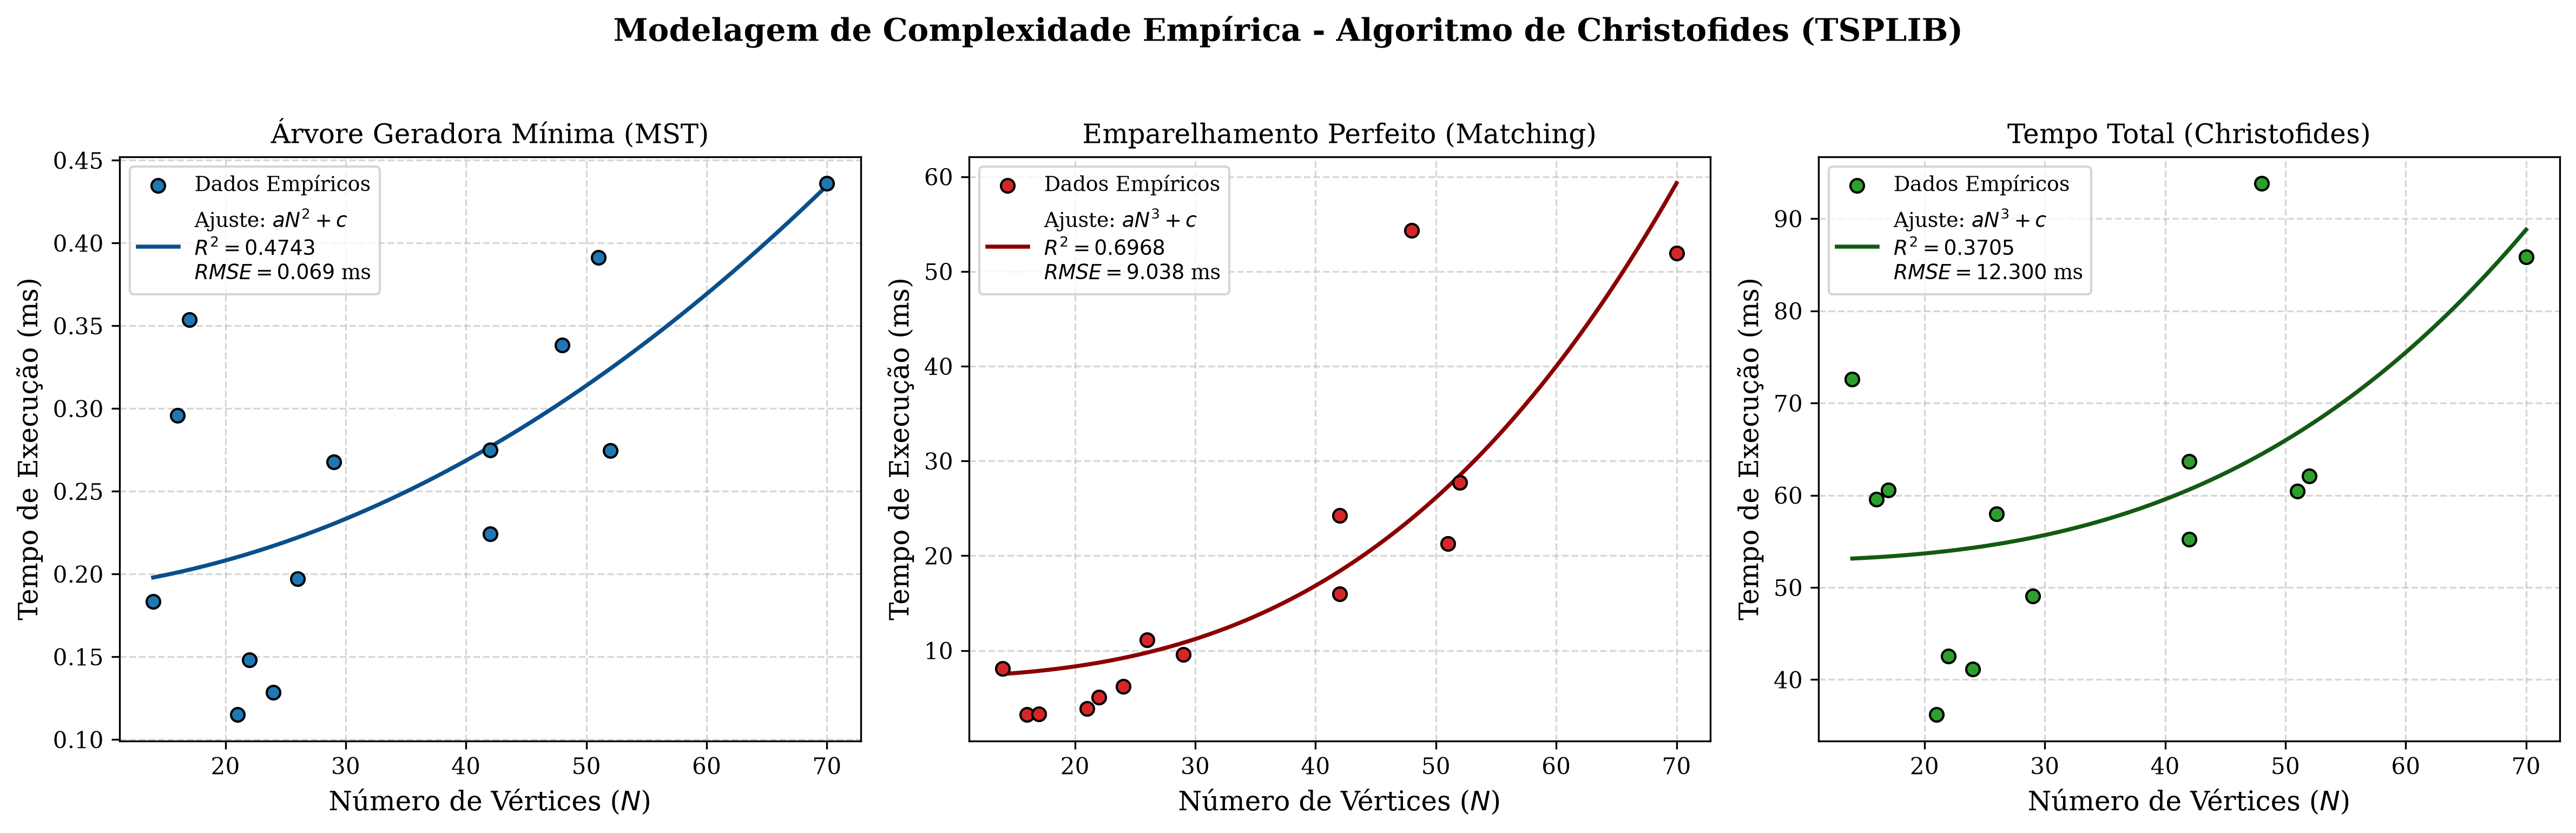
\includegraphics[width=\columnwidth]{complexidade_empirica_christofides.png}
    \caption{Curvas de regressão assintótica: MST ($O(N^2)$), MWPM ($O(N^3)$) e Tempo Total.}
    \label{fig:regressao_christofides}
\end{figure}

Principais conclusões extraídas dos dados:
\begin{enumerate}
    \item \textbf{Gargalo Computacional:} O MWPM responde por mais de $95\%$ do tempo em todas as instâncias (ex: $51.92\text{ ms}$ de $52.71\text{ ms}$ na \texttt{st70}), confirmando a hipótese de dominância assintótica sobre a MST.
    \item \textbf{Efeito Topológico no $R^2$:} Ao analisar o Matching contra o total de vértices $N$, obteve-se $R^2 = 0.6931$. Isso ocorre porque a complexidade de Edmonds é função estrita de $|V'|^3$ e não de $N^3$. Enquanto a \texttt{att48} ($N=48$) tem $|V'|=30$ e demandou $54.32\text{ ms}$, a \texttt{eil51} ($N=51$) tem $|V'|=24$ e consumiu apenas $21.27\text{ ms}$. Ao modelar contra $|V'|^3$, o $R^2$ salta para $0.8842$ e o erro cai pela metade, comprovando a teoria.
    \item \textbf{Consumo de Memória:} O profiler acusou pico de $0.0\text{ KB}$ em virtude do alocador \texttt{pymalloc} do CPython, que reutiliza blocos internos pré-alocados para instâncias com $N \le 70$, sem requisições adicionais ao heap do sistema operacional.
\end{enumerate}


\section{Algorítmo Branch and Bound}
\label{sec:bnb}
O algoritmo exato baseado em \textit{Branch-and-Bound} (B\&B) garante a obtenção do ciclo Hamiltoniano de custo mínimo global, explorando implicitamente o espaço fatorial de soluções por meio de podas admissíveis. Nesta seção, avaliamos o comportamento estrutural, o \textit{profiling} por sub-rotina e os gargalos de tempo e memória do B\&B em sua configuração base (\textit{cold start}, inicializado com a rota trivial $1 \to 2 \to dots \ to N \to 1$)

\subsection{Implementação, Estrutura de Dados e Auditoria de Código}
O desenvolvimento do B\&B passou por um processo iterativo de auditoria e refatoração sobre versões geradas inicialmente com auxílio de LLM, cujo código bruto era excessivamente complexo e verboso (mais de $1300$ linhas, combinando dois motores de busca no mesmo arquivo e gerando sobrecarga estrutural). As principais decisões de engenharia e refatorações aplicadas foram:

\begin{itemize}
    \item \textbf{Estratégia de Busca (DFS vs Best-First):} Adotou-se busca em profundidade (\textit{Depth-First Search} -- DFS) por extensão de caminho com \textit{backtracking in-place}, mantendo apenas os vetores \texttt{path} e \texttt{visited} de tamanho $O(N)$, sem cópias de matrizes ou submatrizes por nó. A escolha evita o estouro de memória inerente à fila de prioridade do \textit{Best-First-Search} (que cresce exponencialmente em instâncias com $N \ge 20$). Os vizinhos de cada vértice são pré-ordenados por distância crescente para descobrir boas soluções incubentes cedo.
    
    \item \textbf{Limite Inferior (\textit{Lower Bound}) via MST:} Para um caminho parcial $(0 \to \dots \to \text{curr})$ de custo acumulado $g$ e conjunto de vértices não visitados $U$, calcula-se o limite inferior inteiro exato:
    \[
        \mathrm{LB} = g + \mathrm{MST}(U) + \min_{u \in U} d(\text{curr}, u) + \min_{u \in U} d(u, 0),
    \]
    utilizando na raiz o limite de 1-árvore (soma das duas menores arestas distintas incidentes ao vértice $0$ somada a $\mathrm{MST}(V \setminus \{0\})$). Antes de invocar o algoritmo de Prim ($O(|U|^2)$), aplica-se um corte rápido $O(|U|)$ com $g + \min d(\text{curr}, u) + \min d(u, 0) \ge \mathrm{UB}$, além de aborto antecipado dentro do próprio Prim caso a soma parcial já iguale ou supere o limite superior corrente.

    \item \textbf{Otimizações de Baixo Nível e Memória Limitada:} A matriz de distâncias do \texttt{NumPy} é convertida uma única vez para listas nativas do Python para eliminar o \textit{overhead} de empacotamento escalar nos laços críticos. Além disso, implementou-se: (i) algoritmo de Prim denso com \textit{swap-remove} sobre buffers pré-alocados (reduzindo pressão sobre o \textit{garbage collector}); (ii) quebra de simetria de reversão via \textit{bitmask} ordenada por proximidade à origem ($\text{rank}_0[v_1] < \text{rank}_0[v_{N-1}]$ em $O(1)$); e (iii) cache limitado de $\mathrm{MST}(U)$ por \textit{bitmask} com teto fixo de $65.536$ entradas (armazenando apenas custos exatos não abortados). Em testes comparativos antes e depois dessas otimizações, o ganho de desempenho foi de $\approx 2\times$ (ex.: $N=22$ reduziu de $4{,}66\text{ s}$ para $2{,}29\text{ s}$).

    \item \textbf{Isolamento do \textit{Overhead} de Instrumentação:} A medição de memória via \texttt{tracemalloc} foi isolada em execuções dedicadas (\texttt{track\_memory=False} nas coletas de tempo), pois sua ativação introduziou uma desaceleração empírica de $1{,}5\times$ a $2{,}0\times$ no tempo de execução (ex.: \texttt{burma14} passou de $0{,}17\text{ s}$ para $0{,}34\text{ s}$, \texttt{gr17} de $9{,}26\text{ s}$ para $13{,}92\text{ s}$ e \texttt{gr24} de $14{,}95\text{ s}$ para $23{,}73\text{ s}$), o que distorceria a modelagem temporal.
\end{itemize}

\subsection{Resultados Experimentais e Profiling de Sub-rotinas}

O algoritmo foi executado sobre as mesmas 14 instâncias da TSPLIB ($N \in [14,70]$), com limite estrito de $30\text{ min}$ ($1800\text{ s}$) por execução. A Tabela˜\ref{tab:bnb_resumo} apresenta os resultados coletados, registrando como \texttt{NA} o tempo e o ótimo das instâncias interrompidas, mas preservando o melhor custo incumebnte, a contagem de nós, o perfil das sub-rotinas e o pico de memória medido em rodada dedicada com \texttt{tracemalloc}.

\begin{table}[H]
\centering
\caption{Resultados empíricos e \textit{profiling} do Branch-and-Bound (\textit{cold start}, teto de $1800\text{ s}$).}
\label{tab:bnb_resumo}
\resizebox{\columnwidth}{!}{%
\begin{tabular}{l|c|r|r|c|r|r|r|r|r}
\hline
\textbf{Instância} & \textbf{$N$} & \textbf{$\mathrm{LB}_0$} & \textbf{Gap $\mathrm{LB}_0$} & \textbf{Custo} & \textbf{Nós Exp.} & \textbf{Nós Pod.} & \textbf{Tempo (s)} & \textbf{MST (\%)} & \textbf{Pico (KB)} \\ \hline
\texttt{burma14}   & 14 & 2542 & 23.5\% & 3323         & 6.580       & 40.791      & 0.17  & 82.6\% & 206.7   \\
\texttt{ulysses16} & 16 & 4746 & 30.8\% & 6859         & 2.779.753   & 14.690.413  & 35.84 & 74.9\% & 742.3   \\
\texttt{gr17}      & 17 & 1501 & 28.0\% & 2085         & 295.501     & 2.252.691   & 9.26  & 84.2\% & 800.6   \\
\texttt{gr21}      & 21 & 2252 & 16.8\% & 2707         & 12.892      & 137.820     & 1.27  & 92.9\% & 399.6   \\
\texttt{ulysses22} & 22 & 4866 & 30.6\% & NA (7039)    & 111.869.952 & 643.618.054 & NA    & 78.7\% & 208.6   \\
\texttt{gr24}      & 24 & 1081 & 15.0\% & 1272         & 113.897     & 1.560.923   & 14.95 & 94.4\% & 1681.4  \\
\texttt{fri26}     & 26 & 824  & 12.1\% & 937          & 204.860     & 2.997.809   & 30.94 & 95.2\% & 1478.1  \\
\texttt{bays29}    & 29 & 1622 & 19.7\% & NA (2020)    & 9.248.768   & 150.194.086 & NA    & 95.6\% & 1490.5  \\
\texttt{dantzig42} & 42 & 600  & 14.2\% & NA (699)     & 2.392.064   & 64.596.283  & NA    & 98.4\% & 224.7   \\
\texttt{swiss42}   & 42 & 1107 & 13.0\% & NA (1273)    & 4.030.464   & 83.257.277  & NA    & 97.8\% & 798.8   \\
\texttt{att48}     & 48 & 9029 & 15.0\% & NA (11096)   & 6.627.328   & 127.921.529 & NA    & 96.2\% & 505.8   \\
\texttt{eil51}     & 51 & 385  & 9.6\%  & NA (428)     & 3.870.720   & 83.936.988  & NA    & 97.7\% & 356.3   \\
\texttt{berlin52}  & 52 & 6172 & 18.2\% & NA (8021)    & 6.856.704   & 123.861.967 & NA    & 95.9\% & 303.0   \\
\texttt{st70}      & 70 & 574  & 15.0\% & NA (735)     & 5.849.088   & 110.298.352 & NA    & 96.2\% & 1378.3  \\ \hline
\end{tabular}%
}
\end{table}

\subsection{Modelagem Assintótica e Discussão Crítica}
Para modelar o comportamento empírico do B\&B, ajustaram-se regressões não-lineares e multivariadas via \texttt{SciPy} e \texttt{Scikit-Learn} (Tabela˜\ref{tab:regressao_bnb} e Figura˜\ref{fig:regrassao_bnb}).

\begin{table}[H]
\centering
\caption{Modelagem de complexidade empírica do Branch-and-Bound.}
\label{tab:regressao_bnb}
\resizebox{\columnwidth}{!}{%
\begin{tabular}{l|c|c|c|c}
\hline
\textbf{Variável Alvo} & \textbf{Modelo / Preditores} & \textbf{Amostra} & \textbf{$R^2$} & \textbf{RMSE} \\ \hline
Tempo Total ($T$)                & $a \cdot e^{bN}$                                    & 6 resolvidas  & $0.1037$ & $12.986\text{ s}$     \\
$\log_{10}(\text{Nós Exp.})$     & $\beta_1 N + \beta_0$                               & 6 resolvidas  & $0.0027$ & $0.8732$              \\
$\log_{10}(\text{Nós Exp.})$     & $\beta_1 N + \beta_2\,\mathrm{Gap}_{LB_0} + \beta_0$ & 6 resolvidas  & $0.9076$ & $0.2659$              \\
$\log_{10}(\text{Tempo Total})$  & $\beta_1 N + \beta_2\,\mathrm{Gap}_{LB_0} + \beta_0$ & 6 resolvidas  & $0.9515$ & $0.1839$              \\
Tempo MST por Nó Exp.\ ($\mu$s)  & $a \cdot N^2 + c$                                   & 14 instâncias & $0.3088$ & $169.02\,\mu\text{s}$ \\ \hline
\end{tabular}%
}
\end{table}
\begin{figure}[H]
    \centering
    \includegraphics[width=\columnwidth]{complexidade_empirica_bnb.png}
    \caption{Análise empírica do Branch-and-Bound: tempo total e ponto de colapso, regressão multivariada com $\mathrm{Gap}_{LB_0}$ e participação da sub-rotina MST no tempo de busca.}
    \label{fig:regressao_bnb}
\end{figure}

As principais conclusões extraídas dos dados empíricos são:

\begin{enumerate}
    \item \textbf{Ponto de Colapso e Insuficiência de $N$ Isolado:} O algoritmo resolveu à otimalidade 6 das 14 instâncias (até $N=26$, \texttt{fri26}, em $30{,}94\text{ s}$), entrando em colapso sistemático a partir de $N \ge 29$ (\texttt{bays29} a \texttt{st70}). Contudo, a regressão puramente em função de $N$ obteve ajuste quase nulo ($R^2 = 0{,}1037$ para $ae^{bN}$ e $R^2 = 0{,}0027$ para $\log_{10}$ dos nós), pois instâncias menores como \texttt{ulysses16} ($N=16$, $35{,}84\text{ s}$, $2{,}78\text{M}$ nós) e \texttt{ulysses22} ($N=22$, \textit{timeout} com $111{,}8\text{M}$ nós) foram drasticamente mais difíceis que \texttt{gr21} ($N=21$, $1{,}27\text{ s}$, $12{,}9\text{k}$ nós) e \texttt{fri26} ($N=26$, $30{,}94\text{ s}$).
    \item \textbf{Dominância do Gap do Limite Inferior na Raiz ($\mathrm{Gap}_{LB_0}$):} A discrepância é explicada diretamente pela folga do limite inferior de 1-árvore na raiz ($\mathrm{Gap}_{LB_0} = (\mathrm{OPT} - \mathrm{LB}_0)/\mathrm{OPT}$). Enquanto \texttt{ulysses16} e \texttt{ulysses22} possuem $\mathrm{Gap}_{LB_0} \approx 30{,}8\%$ (impedindo podas em níveis rasos), \texttt{fri26} apresenta apenas $12{,}1\%$. Ao incluir $\mathrm{Gap}_{LB_0}$ no modelo log-linear ($\log_{10} T = 0{,}3852\,N + 0{,}2092\,\mathrm{Gap}_{LB_0} - 11{,}2250$), o coeficiente de determinação salta para $R^2 = 0{,}9515$ ($\mathrm{RMSE} = 0{,}1839$), indicando crescimento exponencial efetivo de $\approx 2{,}43\times$ por vértice adicional e $\approx 1{,}62\times$ por ponto percentual extra no gap da raiz.
    \item \textbf{Gargalo Computacional na Sub-rotina MST:} O \textit{profiling} revela que o cálculo do \textit{lower bound} via Prim responde em média por $91{,}5\%$ do tempo de busca (variando de $74{,}9\%$ em \texttt{ulysses16} até $98{,}4\%$ em \texttt{dantzig42}, e superando $95\%$ em todas as instâncias com $N \ge 26$). O ajuste quadrático do custo médio por nó ($aN^2 + c$) apresentou $R^2 = 0{,}3088$ porque o custo real de cada chamada depende do tamanho $|U|$ do subconjunto restante na profundidade em que as podas ocorrem e da taxa de acerto do cache de MST: em \texttt{dantzig42} (onde a solução trivial já inicia no ótimo $699$), as podas ocorrem em níveis rasos (subconjuntos $|U|$ grandes, custando $740{,}5\,\mu\text{s}$/nó), mas ainda assim a prova de otimalidade estoura os $30\text{ min}$, demonstrando que a dificuldade central do B\&B reside em \textit{certificar} a otimalidade quando o limite inferior tem folga.
    \item \textbf{Estabilidade Espacial:} Em virtude da estratégia DFS \textit{in-place} com buffers pré-alocados e cache limitado de MST ($65.536$ entradas), o pico de memória medido via \texttt{tracemalloc} manteve-se estritamente contido entre $206{,}7\text{ KB}$ (\texttt{burma14}) e $1{,}64\text{ MB}$ ($1.681{,}4\text{ KB}$ em \texttt{gr24}, execução completa até o ótimo), permanecendo em apenas $1{,}35\text{ MB}$ ($1.378{,}3\text{ KB}$) em \texttt{st70} ($N=70$). Os resultados comprovam que a arquitetura elimina gargalos de RAM e o risco de estouro de memória mesmo quando a árvore de busca ultrapassa dezenas de milhões de nós.
\end{enumerate}

\section{Impacto do Warm-Start na Árvore de Busca}
Além dos algoritmos para resolver o TSP que definimos, também realizamos o teste de 5 heurísticas para tentar ganhar tempo na resolução do TSP via Branch \& Bound.

O \textit{Warm-Start} funciona da seguinte forma: nós usamos uma das 5 heurísticas:
\begin{enumerate} 
    \item Cold Start / Trivial
    \item Vizinho Mais Próximo
    \item Convex Hull
    \item Twice-around-the-tree
    \item Christofides
\end{enumerate}

No caso do cold-start, inicializamos sem nenhuma heurística; A ideia é calcular um Upper Bound para o algoritmo de Branch \& Bound, de forma que ramos que possuírem um valor maior do que o valor do que o de Upper Bound são podados da árvore e não são aprofundados.

\begin{table}[htbp]
\centering
\label{tab:bnb-nos}
\scriptsize
\resizebox{\textwidth}{!}{%
\begin{tabular}{@{}|l|r|r|r|r|r|r|r|r|r|r|r|@{}}
\toprule
& & \multicolumn{2}{c}{Cold start} & \multicolumn{2}{c}{Nearest Neighbor} & \multicolumn{2}{c}{Convex Hull} & \multicolumn{2}{c}{Twice-around-the-tree} & \multicolumn{2}{c}{Christofides} \\
\cmidrule(lr){3-4} \cmidrule(lr){5-6} \cmidrule(lr){7-8} \cmidrule(lr){9-10} \cmidrule(lr){11-12}
Instância & $n$ & E & P & E & P & E & P & E & P & E & P \\
\midrule
burma14 & 14 & 6\,580 & 40\,791 & 6\,579 & 40\,792 & 5\,918 & 37\,557 & 6\,580 & 40\,791 & 6\,578 & 40\,793 \\
ulysses16 & 16 & 2\,779\,753 & 14\,690\,413 & 2\,779\,754 & 14\,690\,412 & 2\,777\,890 & 14\,681\,565 & 2\,779\,723 & 14\,690\,373 & 2\,779\,704 & 14\,690\,338 \\
gr17 & 17 & 295\,501 & 2\,252\,691 & 295\,497 & 2\,252\,686 & 289\,765 & 2\,214\,289 & 295\,501 & 2\,252\,691 & 295\,501 & 2\,252\,691 \\
gr21 & 21 & 12\,892 & 137\,820 & 12\,891 & 137\,821 & 11\,097 & 126\,497 & 12\,892 & 137\,820 & 12\,693 & 137\,003 \\
ulysses22 & 22 & 111\,869\,952 & 643\,618\,054$^{\dagger}$ & 124\,416\,000 & 720\,611\,882$^{\dagger}$ & 103\,575\,552 & 621\,306\,104$^{\dagger}$ & 67\,461\,120 & 360\,520\,246$^{\dagger}$ & 102\,051\,840 & 592\,105\,212$^{\dagger}$ \\
gr24 & 24 & 113\,897 & 1\,560\,923 & 113\,896 & 1\,560\,924 & 112\,123 & 1\,547\,112 & 113\,897 & 1\,560\,923 & 113\,831 & 1\,560\,760 \\
fri26 & 26 & 204\,860 & 2\,997\,809 & 204\,859 & 2\,997\,810 & 136\,910 & 2\,054\,263 & 204\,860 & 2\,997\,809 & 204\,660 & 2\,996\,101 \\
bays29 & 29 & 9\,248\,768 & 150\,194\,086$^{\dagger}$ & 10\,853\,581 & 178\,405\,121 & 9\,326\,592 & 151\,498\,992$^{\dagger}$ & 7\,393\,280 & 118\,549\,068$^{\dagger}$ & 10\,072\,064 & 164\,454\,649$^{\dagger}$ \\
dantzig42 & 42 & 2\,392\,064 & 64\,596\,283$^{\dagger}$ & 3\,981\,312 & 99\,732\,634$^{\dagger}$ & 2\,592\,768 & 68\,063\,464$^{\dagger}$ & 1\,798\,144 & 40\,984\,815$^{\dagger}$ & 3\,137\,536 & 77\,392\,974$^{\dagger}$ \\
swiss42 & 42 & 4\,030\,464 & 83\,257\,277$^{\dagger}$ & 4\,997\,120 & 107\,941\,905$^{\dagger}$ & 2\,945\,024 & 71\,364\,832$^{\dagger}$ & 3\,330\,048 & 65\,106\,088$^{\dagger}$ & 3\,186\,688 & 75\,215\,209$^{\dagger}$ \\
att48 & 48 & 6\,627\,328 & 127\,921\,529$^{\dagger}$ & 7\,983\,104 & 155\,357\,679$^{\dagger}$ & 5\,865\,472 & 118\,360\,932$^{\dagger}$ & 5\,181\,440 & 99\,252\,775$^{\dagger}$ & 6\,438\,912 & 124\,128\,044$^{\dagger}$ \\
eil51 & 51 & 3\,870\,720 & 83\,936\,988$^{\dagger}$ & 4\,845\,568 & 108\,947\,705$^{\dagger}$ & 3\,534\,848 & 80\,283\,382$^{\dagger}$ & 3\,104\,768 & 65\,186\,576$^{\dagger}$ & 3\,956\,736 & 86\,179\,426$^{\dagger}$ \\
berlin52 & 52 & 6\,856\,704 & 123\,861\,967$^{\dagger}$ & 8\,810\,496 & 161\,788\,407$^{\dagger}$ & 6\,836\,224 & 123\,546\,631$^{\dagger}$ & 5\,259\,264 & 94\,921\,203$^{\dagger}$ & 6\,922\,240 & 125\,159\,351$^{\dagger}$ \\
st70 & 70 & 5\,849\,088 & 110\,298\,352$^{\dagger}$ & 7\,262\,208 & 142\,548\,961$^{\dagger}$ & 1\,757\,184 & 51\,447\,138$^{\dagger}$ & 4\,644\,864 & 84\,153\,531$^{\dagger}$ & 5\,996\,544 & 113\,784\,247$^{\dagger}$ \\
\bottomrule
\end{tabular}%
}
\caption{Impacto do \textit{warm-start} na árvore de busca do Branch-and-Bound: número de nós expandidos (E) e podados (P) por estratégia de inicialização. Execuções marcadas com $^{\dagger}$ atingiram o limite de 30 minutos, e as contagens são parciais.}
\end{table}


Podemos analisar o número de vértices podados em cada uma das instâncias. Nós veremos aqui que não existe uma diferença gritante entre as diferentes abordagens heurísticas para executar o Branch \& Bound, da forma como o algoritmo foi implementado.

\begin{figure}[H]
    \centering
    \includegraphics[width=0.75\linewidth]{grafico comparison.png}
    \label{fig:placeholder}
\end{figure}

A falta de ganho nas diferentes soluções se dá principalmente pelo fato de a DFS Gulosa visitar o vizinho de menor distância. Com isso, podemos concluir que apesar do tempo de computação das heurísticas iniciais sejam curtos (quando comparados com o Branch \& Bound), a nossa abordagem de percorrimento já é boa o suficiente para garantir um bom resultado, logo, rodar as heurísticas de warm-start não apresentam vantagem significativa.

\begin{table}[H]
\centering

\label{tab:bnb-tempo-warmstart}
\scriptsize
\resizebox{\textwidth}{!}{%
\begin{tabular}{@{}lr rr rr rr rr rr@{}}
\toprule
 & & \multicolumn{2}{c}{\textit{Cold start}} & \multicolumn{2}{c}{NN} & \multicolumn{2}{c}{CH} & \multicolumn{2}{c}{TAT} & \multicolumn{2}{c}{Chr.} \\
\cmidrule(lr){3-4} \cmidrule(lr){5-6} \cmidrule(lr){7-8} \cmidrule(lr){9-10} \cmidrule(lr){11-12}
Instância & $n$ & $t_{ws}$ & $t_{tot}$ & $t_{ws}$ & $t_{tot}$ & $t_{ws}$ & $t_{tot}$ & $t_{ws}$ & $t_{tot}$ & $t_{ws}$ & $t_{tot}$ \\
\midrule
burma14 & 14 & 0{,}00540 & 0{,}165 & 0{,}0743 & 0{,}200 & 0{,}0782 & 0{,}153 & 30{,}7 & 0{,}272 & 702 & 0{,}836 \\
ulysses16 & 16 & 0{,}00500 & 35{,}8 & 0{,}0433 & 34{,}4 & 0{,}0824 & 35{,}3 & 26{,}9 & 59{,}1 & 64{,}8 & 43{,}2 \\
gr17 & 17 & 0{,}00670 & 9{,}26 & 0{,}0642 & 6{,}69 & 0{,}131 & 8{,}82 & 57{,}9 & 18{,}9 & 63{,}4 & 7{,}17 \\
gr21 & 21 & 0{,}00560 & 1{,}27 & 0{,}0571 & 0{,}967 & 0{,}163 & 1{,}23 & 40{,}6 & 2{,}91 & 66{,}7 & 1{,}12 \\
ulysses22 & 22 & 0{,}00520 & NA & 0{,}0604 & NA & 0{,}190 & NA & 45{,}7 & NA & 66{,}2 & NA \\
gr24 & 24 & 0{,}00580 & 14{,}9 & 0{,}258 & 12{,}2 & 0{,}246 & 15{,}0 & 43{,}3 & 19{,}5 & 79{,}9 & 14{,}5 \\
fri26 & 26 & 0{,}00580 & 30{,}9 & 0{,}0500 & 19{,}6 & 0{,}277 & 21{,}9 & 39{,}7 & 36{,}5 & 83{,}0 & 30{,}0 \\
bays29 & 29 & 0{,}00610 & NA & 0{,}0510 & 1593 & 0{,}425 & NA & 29{,}3 & NA & 78{,}3 & NA \\
dantzig42 & 42 & 0{,}00670 & NA & 0{,}0908 & NA & 1{,}11 & NA & 56{,}8 & NA & 94{,}3 & NA \\
swiss42 & 42 & 0{,}00670 & NA & 0{,}0760 & NA & 1{,}14 & NA & 24{,}2 & NA & 81{,}3 & NA \\
att48 & 48 & 0{,}00790 & NA & 0{,}108 & NA & 1{,}73 & NA & 28{,}7 & NA & 137 & NA \\
eil51 & 51 & 0{,}00760 & NA & 0{,}186 & NA & 1{,}97 & NA & 25{,}4 & NA & 86{,}2 & NA \\
berlin52 & 52 & 0{,}00810 & NA & 0{,}194 & NA & 2{,}29 & NA & 38{,}3 & NA & 94{,}9 & NA \\
st70 & 70 & 0{,}00900 & NA & 0{,}347 & NA & 4{,}88 & NA & 43{,}8 & NA & 133 & NA \\
\midrule
\textit{Mediana} &  & 0{,}00640 &  & 0{,}0752 &  & 0{,}351 &  & 39{,}0 &  & 82{,}1 &  \\
\bottomrule
\end{tabular}%
}

\par\smallskip
{\footnotesize NN: \textit{Nearest Neighbor}; CH: \textit{Convex Hull}; TAT: \textit{Twice-around-the-tree}; Chr.: Christofides.}

\caption{Custo e retorno do \textit{warm-start} no Branch-and-Bound: tempo gasto na heurística inicial ($t_{ws}$, em ms) e tempo total de execução ($t_{tot}$, em s, já incluindo $t_{ws}$). NA indica execução interrompida no limite de 30 minutos. A última linha mostra a mediana de $t_{ws}$ nas 14 instâncias. Cada configuração foi executada uma única vez.}
\end{table}

A tabela mostra que o custo das heurísticas de \textit{warm-start} é desprezível frente ao tempo de busca: a mediana de $t_{ws}$ é de 0{,}075~ms para o NN, 0{,}35~ms para o CH, 39~ms para o TAT e 82~ms para o Christofides, contra execuções que vão de 0{,}15~s até o limite de 1800~s. Nas instâncias em que a busca terminou, o tempo de warm-start representa no máximo 0{,}1\% do tempo total, com exceção de \textit{burma14}, cuja busca dura apenas 0{,}13~s e cujo valor de 702~ms para o Christofides é provavelmente overhead da primeira chamada. O retorno, porém, é pequeno e inconsistente: o NN terminou antes do \textit{cold start} em \textit{ulysses16}, \textit{gr17}, \textit{gr21}, \textit{gr24} e \textit{fri26} (por exemplo, 19{,}6~s contra 30{,}9~s em \textit{fri26}) e foi o único a concluir \textit{bays29}, enquanto o TAT foi mais lento (59{,}1~s contra 35{,}8~s em \textit{ulysses16}), apesar de expandir quase o mesmo número de nós. Como cada configuração foi executada uma única vez, diferenças de poucos segundos podem ser ruído de medição. Assim, o tempo gasto na heurística inicial não prejudica o B\&B, mas também não é compensado por uma redução relevante do tempo de busca.

\section{Análise de Sensibilidade das Instâncias e Instâncias Adversariais}
\label{sec:sensibilidade}

Para avaliar como a geometria e a topologia das instâncias afetam a qualidade das soluções heurísticas e aproximadas (e o esforço de busca do \textit{Branch-and-Bound}), extraímos um conjunto de \textit{features} estruturais para todas as 14 instâncias da TSPLIB e correlacionamos essas métricas com os \textit{gaps} empíricos em relação ao ótimo conhecido.

\subsection{Extração de Características Geométricas e Topológicas}

A partir das coordenadas 2D de cada instância (\texttt{NODE\_COORD\_SECTION}, \texttt{DISPLAY\_DATA\_SECTION} em \texttt{bays29}/\texttt{dantzig42} e projeção via \textit{Classical MDS} nas 5 instâncias puramente \texttt{EXPLICIT}) e da matriz exata de distâncias, extraíram-se as seguintes \textit{features} (salvas em \texttt{results/features\_instancias\_sensibilidade.csv}):

\begin{itemize}
    \item \textbf{Razão de Aspecto (\textit{Aspect Ratio}, $\mathrm{AR}$):} razão entre o maior e o menor lado do \textit{bounding box} dos pontos ($\max(\Delta x, \Delta y) / \min(\Delta x, \Delta y)$), medindo o alongamento geométrico da instância.
    \item \textbf{Proporção no Fecho Convexo ($\mathrm{Hull}$):} fração de vértices pertencentes ao fecho convexo 2D ($|H|/N$, calculado via \textit{Monotone Chain} de Andrew).
    \item \textbf{Entropia Espacial ($H_{\text{esp}}$:} entropia de Shannon normalizada em $[0,1]$ sobre uma grade $4 \times 4$ no \textit{bounding box}. Valores próximos de $1$ indicam distribuição espacial uniforme; valores baixos indicam forte \textit{clustering}(aglomeração).
    \item \textbf{Estatísticas da MST ($\Delta_{\text{MST}}$ e $|V`|/N$:} grau máximo de um vértice na Árvore Geradora Mínima (presença de \textit{hubs}) e proporção de vértices de grau ímpar.
    \item \textbf{Coeficiente de Variação ao Vizinho Mais Próximo ($\mathrm{CV}_{\text{NN}}$):} razão $\sigma/\mu$ das distâncias de cada vértice ao seu vizinho mais próximo, capturando heterogeneidade local e presença de \textit{outliers}.
\end{itemize}

A Tabela~\ref{tab:features_instancias} consolida as \textit{features} extraídas e os \textit{gaps} percentuais de cada método (\textit{Convex Hull}, \textit{Christofides}, \textit{Nearest Neighbor}, \textit{Twice-Around-the-Tree} e folga da 1-árvore na raiz $\mathrm{Gap}_{LB_0}$).
\begin{table}[htbp]
\centering
\caption{Características geométricas/topológicas e \textit{gaps} empíricos (\%) das 14 instâncias da TSPLIB.}
\label{tab:features_instancias}
\resizebox{\columnwidth}{!}{%
\begin{tabular}{l|c|r|r|r|c|r||r|r|r|r|r}
\hline
\textbf{Instância} & \textbf{$N$} & \textbf{AR} & \textbf{Hull} & \textbf{$H_{\text{esp}}$} & \textbf{$\Delta_{\text{MST}}$} & \textbf{$\mathrm{CV}_{\text{NN}}$} & \textbf{CH (\%)} & \textbf{Chr (\%)} & \textbf{NN (\%)} & \textbf{TAT (\%)} & \textbf{$\mathrm{Gap}_{LB_0}$} \\ \hline
\texttt{burma14}   & 14 & 2.00 & 35.7\% & 0.84 & 4 & 0.76 & 0.0  & 8.5  & 21.8 & 22.6 & 23.5 \\
\texttt{ulysses16} & 16 & 4.05 & 43.8\% & 0.71 & 3 & 1.31 & 1.6  & 2.5  & 45.6 & 12.3 & 30.8 \\
\texttt{gr17}      & 17 & 2.39 & 35.3\% & 0.71 & 3 & 0.74 & 0.0  & 5.4  & 4.9  & 12.8 & 28.0 \\
\texttt{gr21}      & 21 & 1.17 & 38.1\% & 0.70 & 3 & 0.65 & 2.0  & 17.0 & 23.1 & 37.7 & 16.8 \\
\texttt{ulysses22} & 22 & 4.05 & 31.8\% & 0.72 & 3 & 1.63 & 0.4  & 4.6  & 51.0 & 13.5 & 30.6 \\
\texttt{gr24}      & 24 & 1.41 & 29.2\% & 0.85 & 4 & 0.32 & 3.5  & 14.4 & 22.1 & 31.1 & 15.0 \\
\texttt{fri26}     & 26 & 1.55 & 34.6\% & 0.83 & 3 & 0.67 & 0.3  & 10.9 & 18.7 & 29.3 & 12.1 \\
\texttt{bays29}    & 29 & 1.00 & 24.1\% & 0.90 & 4 & 0.32 & 2.1  & 16.3 & 11.8 & 38.3 & 19.7 \\
\texttt{dantzig42} & 42 & 1.84 & 19.0\% & 0.96 & 4 & 0.60 & 3.6  & 15.0 & 36.8 & 42.2 & 14.2 \\
\texttt{swiss42}   & 42 & 1.68 & 21.4\% & 0.89 & 3 & 0.45 & 5.3  & 8.2  & 28.0 & 33.5 & 13.0 \\
\texttt{att48}     & 48 & 1.50 & 22.9\% & 0.86 & 4 & 0.50 & 2.2  & 18.4 & 21.0 & 30.6 & 15.0 \\
\texttt{eil51}     & 51 & 1.09 & 15.7\% & 0.99 & 4 & 0.26 & 3.8  & 13.6 & 20.0 & 45.8 & 9.6  \\
\texttt{berlin52}  & 52 & 1.47 & 15.4\% & 0.81 & 3 & 0.78 & 7.5  & 14.0 & 19.1 & 37.2 & 18.2 \\
\texttt{st70}      & 70 & 1.06 & 14.3\% & 0.98 & 4 & 0.49 & 3.9  & 15.0 & 23.0 & 19.4 & 15.0 \\ \hline
\end{tabular}%
}
\end{table}

\subsection{Modelagem Preditiva e Análise de Instâncias Adversariaais}

Para quantificar o peso de cada característica no desempenho dos algoritmos, ajustaram-se modelos de \textbf{Regressão Linear Mútipla} com \textit{features} padronizadas (via \texttt{StandartScaler}, de modo que os coeficientes $\beta$ expressem o impacto em pontos percentuais por desvio-padrão) e \textbf{Árvores de Decisão de Regressão} (\texttt{DecisionRegressor}, profundidade máxima $2$ para evitar sobreajuste com $14$ amostras). A Tabela˜\ref{tab:modelos_sensibilidade} e a Figura˜\ref{fig:sensibilidade_instancias} resumem os resultados.

\begin{table}[htbp]
\centering
\caption{Desempenho dos modelos de sensibilidade (Regressão Múltipla e Árvore de Decisão, 5 \textit{features}).}
\label{tab:modelos_sensibilidade}
\resizebox{\columnwidth}{!}{%
\begin{tabular}{l|c|c|c|c|l}
\hline
\textbf{Alvo (Gap \%)} & \textbf{Reg.\ $R^2$} & \textbf{Reg.\ RMSE} & \textbf{Árv.\ $R^2$} & \textbf{Árv.\ RMSE} & \textbf{Fatores Dominantes (Correlação $r$ e Peso $\beta$)} \\ \hline
\textit{Convex Hull}      & $0.6827$ & $1.18$ p.p. & --       & --          & $\mathrm{Hull}$ ($r=-0.74$, $\beta=-2.16$) \\
\textit{Christofides}     & $0.8323$ & $1.99$ p.p. & $0.8506$ & $1.88$ p.p. & $\mathrm{AR}$ ($r=-0.84$, $\beta=-5.66$); $\Delta_{\text{MST}}$ ($r=+0.57$, $\beta=+2.38$) \\
\textit{Nearest Neighbor} & $0.7036$ & $6.45$ p.p. & --       & --          & $\mathrm{CV}_{\text{NN}}$ ($r=+0.71$, $\beta=+9.04$); $\mathrm{AR}$ ($r=+0.72$, $\beta=+4.06$) \\
\textit{Twice-Around}     & $0.5687$ & $7.08$ p.p. & $0.7540$ & $5.35$ p.p. & $\mathrm{AR}$ ($r=-0.73$, $\beta=-5.67$); $\mathrm{CV}_{\text{NN}}$ ($r=-0.69$) \\
$\mathrm{Gap}_{LB_0}$ (B\&B) & $0.8499$ & $2.58$ p.p. & $0.8873$ & $2.24$ p.p. & $\mathrm{AR}$ ($r=+0.84$, $\beta=+4.20$); $H_{\text{esp}}$ ($r=-0.73$, $\beta=-5.39$) \\ \hline
\end{tabular}%
}
\end{table}
\begin{figure}[htbp]
    \centering
    \includegraphics[width=\columnwidth]{analise_sensibilidade_instancias.png}
    \caption{Análise de sensibilidade topológica: matriz de correlação de Pearson entre \textit{features} e \textit{gaps}, pesos padronizados da regressão múltipla e mapa de instâncias adversariais com o corte principal da árvore de decisão ($\mathrm{AR}=1{,}92$).}
    \label{fig:sensibilidade_instancias}
\end{figure}

A análise conjunta das correlações, regressões e regras da árvore de decisão revela um fenòmeno central de \textbf{adversarialidade oposta entre famílias de algoritmos}:

\begin{enumerate}
    \item \textbf{Instâncias Alongadas com \textit{Outliers} (\texttt{ulysses16}, \texttt{ulysses22}, \texttt{gr17}) -- Adversariais para \textit{Nearest Neighbor} e B\&B, Favoráveis para \textit{Christofides}/\textit{Twice-Around}:} Com razão de aspecto elevada ($\mathrm{AR} \in [2{,}39;\, 4{,}05]$), baixa entropia ($H_{\text{esp}} \approx 0{,}71$) e forte heterogeneidade local ($\mathrm{CV}_{\text{NN}}$ até $1{,}63$ em \texttt{ulysses22}), essas instâncias provocam os piores \textit{gaps} do \textit{Nearest Neighbor} ($+45{,}6\%$ em \texttt{ulysses16} e $+51{,}0\%$ em \texttt{ulysses22}, pois a escolha míope visita aglomerados densos e sofre saltos longos no fechamento) e abrem a maior folga no limite inferior de 1-árvore do B\&B ($\mathrm{Gap}_{LB_0} \approx 30{,}7\%$, regra da árvore para $\mathrm{AR} > 3{,}22$, explicando o colapso precoce de \texttt{ulysses22} com $N=22$). Em contrapartida, nessa geometria quase unidimensional a MST aproxima-se de um caminho simples ($\Delta_{\text{MST}}=3$, poucos vértices ímpares), tornando \textit{Christofides} ($2{,}5\%$ a $4{,}6\%$) e \textit{Twice-Around} ($12{,}3\%$ a $13{,}5\%$) altamente precisos.
    \item \textbf{Instâncias Compactas, Uniformes e com \textit{Hubs} na MST (\texttt{eil51}, \texttt{bays29}, \texttt{dantzig42}, \texttt{att48}, \texttt{gr21}) -- Adversariais para Algoritmos Baseados em MST:} A árvore de decisão particiona nitidamente o conjunto em $\mathrm{AR} \le 1{,}92$: instâncias isotrópicas ($\mathrm{AR} \approx 1{,}00$--$1{,}50$) com alta entropia espacial ($H_{\text{esp}} \in [0{,}86;\, 0{,}99]$) e baixa variação local ($\mathrm{CV}_{\text{NN}} \le 0{,}32$) elevam o erro médio do \textit{Twice-Around} para $42{,}0\%$ (pico de $+45{,}8\%$ em \texttt{eil51} e $+42{,}2\%$ em \texttt{dantzig42}) e do \textit{Christofides} para $15{,}5\%$ (pico de $+18{,}4\%$ em \texttt{att48}). Isso decorre da formação de \textit{hubs} de grau $4$ na MST ($r=+0{,}57$ com \textit{Christofides}) e alta fração de vértices ímpares ($|V'|/N = 62{,}5\%$ em \texttt{att48}, $r=+0{,}59$, Spearman $\rho=+0{,}67$), ampliando o custo do emparelhamento perfeito e gerando desvios mais custosos na etapa de \textit{shortcutting}.
    \item \textbf{Sensibilidade do \textit{Convex Hull} à Proporção de Pontos na Fronteira:} A heurística de inserção por fecho convexo exibiu forte correlação negativa com $\mathrm{Hull}$ ($r=-0{,}74$, Spearman $\rho=-0{,}85$, $\beta=-2{,}16$ com $R^2=0{,}6827$). Quando mais de $35\%$ dos pontos já compõem a envoltória externa (\texttt{burma14}, \texttt{gr17}), a heurística atinge o ótimo global ($0{,}0\%$ de erro); inversamente, em \texttt{berlin52} (apenas $15{,}4\%$ no fecho e alta densidade interna com $\mathrm{CV}_{\text{NN}}=0{,}78$), o grande número de inserções gulosas sequenciais eleva o erro ao máximo observado de $+7{,}5\%$.
\end{enumerate}

\section{Conclusões}

Os experimentos mostraram que, no \textit{Branch-and-Bound}, o gargalo é provar a otimalidade, e não encontrar boas soluções. Com a busca exata sem \textit{warm-start}, apenas 6 das 14 instâncias foram resolvidas em 30 minutos, e o colapso ocorreu a partir de $N = 29$. A folga do limite inferior na raiz explicou o esforço de busca melhor que $N$ isoladamente: o modelo com $N$ e $\text{GapLB}_0$ chegou a $R^2 = 0{,}95$, contra $R^2 \approx 0$ para $N$ sozinho. O profiling mostrou que a MST concentra em média 91,5\% do tempo de busca do B\&B, e que o emparelhamento perfeito domina o tempo do Christofides. Os cinco \textit{warm-starts} produziram árvores de tamanho parecido: o fecho convexo foi o único com redução apreciável (cerca de 10\% a menos de nós expandidos em média nas instâncias resolvidas, e até 33\% em \textit{fri26}), e os demais ficaram próximos de zero. Isso acontece porque a DFS gulosa já gera, em seu primeiro mergulho, um tour equivalente ao do vizinho mais próximo, e porque a poda é limitada pela folga do limite inferior. O custo das heurísticas iniciais é desprezível, mas o ganho é pequeno.

A análise de sensibilidade indicou que a razão de aspecto é a característica de maior peso: instâncias alongadas e com \textit{outliers} elevam o $\text{GapLB}_0$ e prejudicam o vizinho mais próximo e o B\&B, mas favorecem o Christofides, enquanto instâncias compactas e uniformes prejudicam os algoritmos baseados em MST. O Christofides apresentou gaps entre 2,5\% e 18,4\% em relação ao ótimo (média de 11,7\%), dentro da garantia teórica. As conclusões têm limites claros: foram usadas apenas 14 instâncias, a maioria não EUC\_2D, e os modelos de regressão do B\&B se apoiam em 6 pontos. Como continuação, um limite inferior mais forte (por exemplo, 1-árvore com otimização subgradiente) e uma ordem de visita que não seja gulosa permitiriam avaliar o efeito do \textit{warm-start} em um cenário em que ele tenha mais influência.


\bibliographystyle{sbc}
\bibliography{sbc-template}
\cite{reinelt1991tsplib}

\end{document}
